\subsection{Introduction}

The team decided it would be in the best interests of the application if we had
real world data and enough of it to properly test the capabilities of the
algorithm. The process unfortunately involved a lot of manual copy and pasting
due to the formatting and structure of the information on the website used with
at most only two days worth of matches being shown on the same page.

Eventually the source file, after having the entire seasons match line up and
information appended continually to it, was finished but still had unnecessary
columns. This was solved by taking the source file, placing it into Microsoft
Excel, selecting the entire redundant columns and simply removing them leaving
only the relevant information. This, along with a few tweaks to get rid of
hidden characters taken from the formatting of the website, left us with a
reliable source of baseball's entire 2012 season information to pass into the
program.

The reasoning behind using 2012's season information was because we discovered
at the start of the project, the season was just finishing as it had ran since
April and it wouldn't be starting again until April 2013. This meant that it
wouldn't run throughout the same time frame we would have to complete the
project. If it had this would have allowed us to actively, in real time, update
the system day by day as the results of matches were published. This was the
main reasoning behind the teams decision in the second semester to instead drop
the future work plan of creating a web based parser that would have made use of
some variation of an RSS feed or an HTML page to extract recent match
information continually.

There was no time overlap to allow real data to be parsed so we looked into
using the next closest sport in terms of the point system; Basketball due to it
having a season running alongside the project time frame in part. The team
ultimately decided to throw this out due to small discrepancies that made it
less viable to use such as 2-1-0 point scoring instead of baseballs 1-0, not to
mention that a lot of time would be spent making the parser come to fruition
when we could use the time to make more features within the desktop application
and ultimately the creation of the web application.

Regardless these were the main reasons behind the teams decision to instead work
retrospectively over a finished season; it allowed us to know the conclusions
for the end of season scores showing that the algorithm did in fact truly work
when it was completed due to the data matching up and it also allowed the
application to test an entire season right from the beginning to check it's
speed capabilities with a full data set.

\subsection{Design}

The design of the parser required figuring out which classes needed to be
created in order to pass information to the algorithm and the user interface,
essentially the backbone of the entire application. Once these were established
and implemented the match information was to flow externally from a specifically
structured source text file, user specified or 2012's default season otherwise.
Once the information had been successfully read in, parsed and stored it would
populate the main classes within the program and could be used by either the
algorithm or the user interface whenever required. The other task was to make
more functionality within the main classes such that the coding by the other
components could be simplified to function calls as extra functionality would
exist to support them.

\subsection{Implementation}

The main classes were identified as Division, Match and Team with the Parser
class being metaphorical funnel that pours information into these classes.
Initially starting out by scanning line by line the provided source file until
it reaches the end having created appropriate objects and stored the relevant
information during the process.

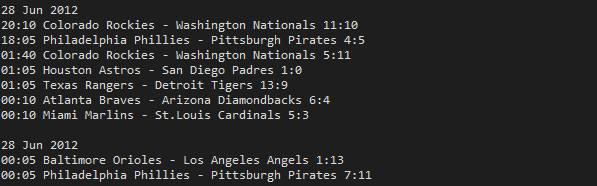
\includegraphics[width=\linewidth,keepaspectratio]{images/sourceFileExample.png}

As can be seen in the screen-shot above this is a sample of data from the 2012
source file. The structure of each line below the date is as follows;

\begin{verbatim}
Time 	Home team - Away team 	Home Score:Away Score
\end{verbatim}

The parser will determine whether it's on a new date or a match and dependant on
which will call the appropriate function that will go a layer deeper and perform
string manipulation to split apart, analyse each individual piece, store and/or
create objects for in the appropriate classes before finishing up and moving
onto the next line in the file should it be a new date or match.

To go more in-depth, the parser must first initialise the 6 available baseball
divisions that exist such as ``American Central'' or ``National West'', by
manually hard-coding their names and the names of the 5 teams associated with
each division because there is no other way to set up the divisions
automatically from an external source. These populated division objects along
with the team objects are stored together in a easily accessible hash map and
from here the parser moves onto it's main functionality as shown by the
following pseudo-code:

\IncMargin{2em}
\begin{algorithm}
  \SetAlgoLined
  \SetKwData{Date}{Date} \SetKwData{Match}{Match}
  \SetKwData{File}{File} \SetKwData{Line}{Line}
  \SetKwData{Teams}{Teams} \SetKwData{Division}{Division}
  \SetKwInOut{Input}{input}

  \Input{A file \File to be parsed}
  \Date $\leftarrow$ a date object used in creating a \Match\;
  \Begin{
      \While{not at end of \File}{
        \Line $\leftarrow$ tokens of next line read from \File\;
        \uIf{\Line is a date}{
          \Date $\leftarrow$ extracted information from \Line\;
        }
        \uElseIf{\Line is a match}{
          \Match $\leftarrow$ extracted information about match from
          \Line\;
          date of \Match $\leftarrow$ \Date\;
          add \Match to upcoming games of the participating \Teams\;
          add \Match to fixtures of respective \Division\;
        }
        \Else{
          Badly formatted input, ignore\;
        }
      }
    }
    \caption{Parser}\label{PARSER}
\end{algorithm}
\DecMargin{2em}

\clearpage